\section{Vybrané distribuované algoritmy}

V našom ponímaní distribuovaných algoritmov, máme nasledovný výpočtový model \cite{tel2000}.
Uvažujme niekoľko počítačov, z ktorých sú niektoré dvojice spojené obojsmernou komunikačnou linkou.
Inak povedané, počítače tvoria neorientovaný graf. Navyše kvôli povahe samotných algoritmov zväčša vyžadujeme,
aby bol graf súvislý. Počet počítačov budeme označovať $n$ a počet liniek $m$.

Do každého z týchto počítačov sa nahrá ten istý program a všetky sa naraz spustia. Programy si môžu
interne čokoľvek počítať a zároveň dokážu poslať správu po ľubovoľnej linke. O správach na linkách
vieme len to, že v konečnom čase dorazia na druhý koniec, a keď jeden počítač pošle po jednej linke
viac správ, tak dorazia v tom istom poradí, v akom boli poslané. O poradí doručenia správ na rôznych
linkách nevieme povedať nič a každá správa sa môže doručovať ľubovoľne dlho. Nemáme teda žiadne garancie, či
správa dorazí do desať minút a kľudne sa môže stať, že niektoré správy prejdú tisícky hrán, zatiaľ čo
iné len jednu.

Dôležitý parameter pri návrhu algoritmu pracujúcom v tomto modeli, je celkový počet odoslaných
správ. Pochopiteľne, sa snažíme aby sa v najhoršom prípade poslalo čo najmenej
správ.

Momentálne sú v aplikácii implementované vizualizácie troch algoritmov.

\subsection{Broadcast}

Jedným z jednoduchších problémov, ktoré treba v distribuovaných algoritmoch riešiť, je, ako 
oznámiť nejakú správu všetkým počítačom (nielen susedom). Keď všetky počítače naštartujú, 
jeden z nich má nejakú informáciu a ostatné by sa ju tiež radi dozvedeli.

Problém sa rieši pomerne priamočiaro, prvý počítač pošle správu všetkým susedom, a každý
počítač, ktorý dostane správu, najprv skontroluje, či už niekedy správu posielal. 
Ak ju ešte neposielal, pošle ju všetkým susedom s výnimkou toho, od ktorého správa prišla.

Takto po každej linke prejde najviac jedna správa, čím dosiahneme optimálny výsledok $O(m)$ správ.

\noindent
\begin{figure*}
\centering
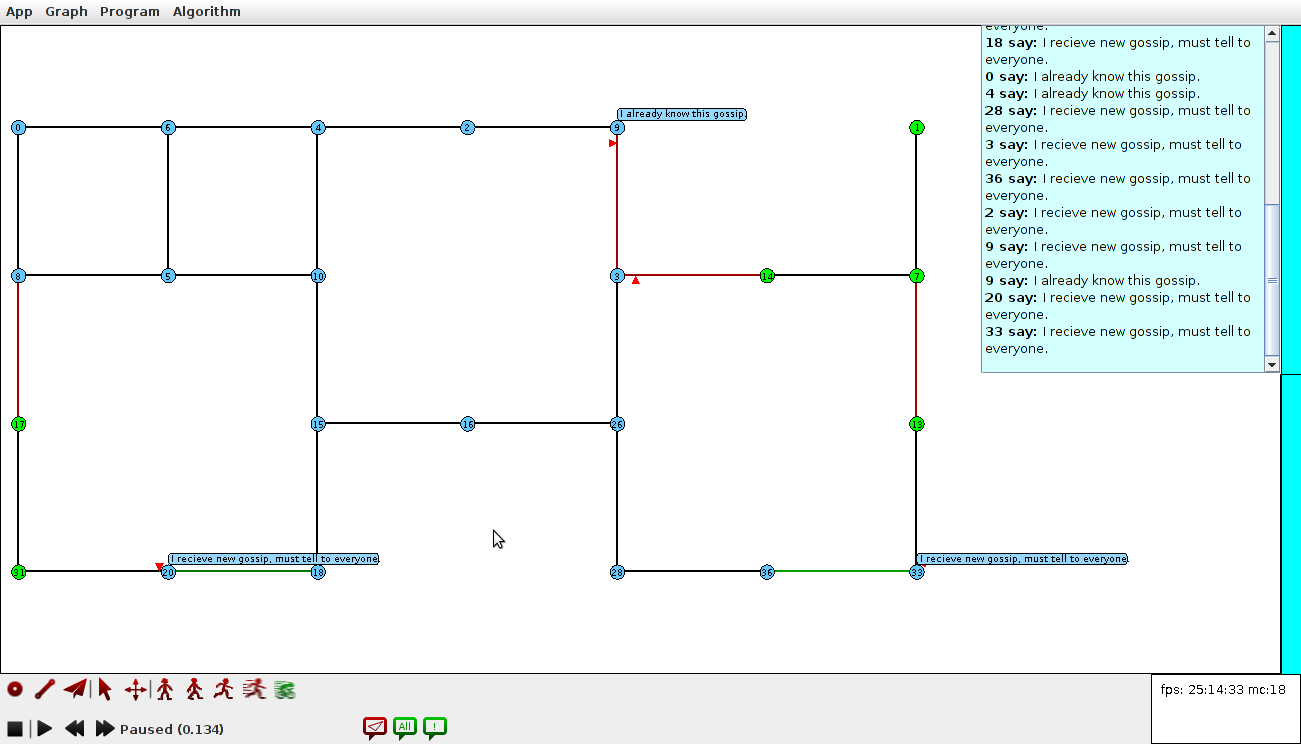
\includegraphics[width=2.01\columnwidth]{BFS.png}
\caption{\emph{Softvér ViDA.} Algoritmus BFS. Svetlomodré vrcholy označujú, že už počuli novú správu,
zelené na ňu zatiaľ čakajú. Vpravo je odkrytý panel, kde si užívateľ môže prezrieť históriu výpisov.}
\label{img:historia} 
\end{figure*}
%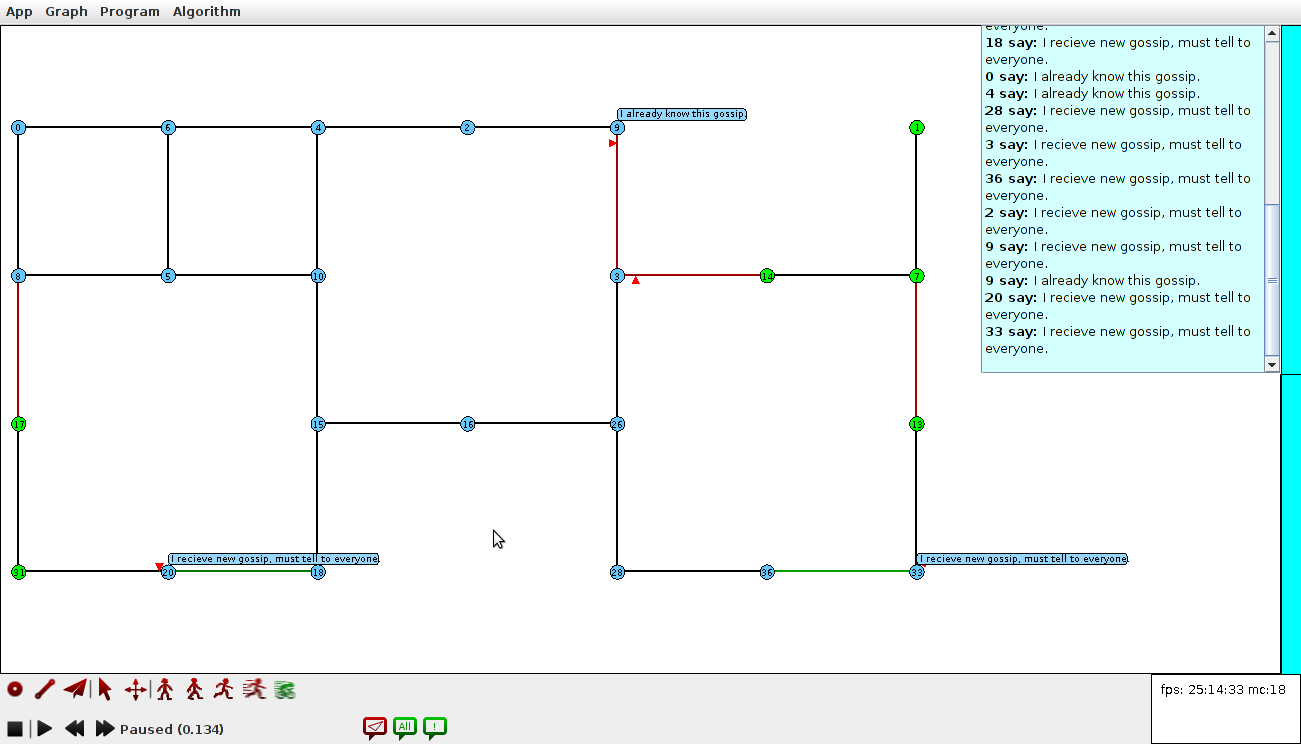
\includegraphics[width=8.5cm]{BFS.png}

\subsection{Voľba šéfa na $n$-vrcholovom úplnom grafe s počtom správ $O(n\log n)$}

Ako názov naznačuje, v tejto sekcii budú všetky dvojice počítačov spojené linkou. 
Navyše má každý počítač svoj jednoznačný identifikátor (ľubovoľné celé číslo, nazvime ho $id$), bez identifikátorov
by sa totiž problém nedal riešiť kvôli symetrii.

Počítače na začiatku poznajú len svoje $id$ a vidia $n-1$ portov očíslovaných číslami $1$ až $n-1$ v
ľubovoľnom poradí (nevedia teda za akým portom je aký počítač). Následne sú programy spustené a môžu začať posielať správy.
Chceme nájsť taký algoritmus, ktorý pre ľubovoľné identifikátory, časovanie správ a poradie
portov, vždy skončí tak, že práve jeden počítač bude vedieť o sebe, že je šéf a ostatné budú vedieť, že nie sú šéfovia.

Dá sa dokázať, že každý takýto algoritmus musí poslať aspoň $O(n\log n)$ správ a my si povieme o
jednom z takých, ktoré to dokážu.

V popise použijeme trocha stredovekú terminológiu. Počítače medzi sebou obrazne bojujú a snažia
sa stať panovníkom čo najväčšieho počtu iných počítačov -- tí sa im stanú vazalmi. 
Počítače môžu vyzvať iný počítač na súboj, a ak vyzývateľ vyhrá, porazený sa stáva jeho vazalom.

Na to, aby sa počítač stal šéfom, musí mať $n-1$ vazalov (teda musí
poraziť všetky ostatné počítače) a sám nesmie byť nikomu vazalom. Každý počítač je vazalom najviac 
jedného počítača. Z tohto vyplyva, že šéf bude najviac jeden. Navyše si označme level $=$ počet vazalov.

Na začiatku sa chce každý počítač stať šéfom a teda snaží sa postupne získať vazalov. Pri každom
pokuse o získanie vazala pošle nejakému z tých susedov, ktorých ešte nevyzýval, správu \verb!"Mám level x, id y a chcem ťa zajať."! 

Ak sused už nie je vazalom niekoho iného, lexikograficky porovná svoju dvojicu $(level, id)$ s
dvojicou zo správy. 
Ak je jeho dvojica väčšia, správu ignoruje a teda pôvodný počítač nikdy nezajme všetkých, čím
zahynie jeho šanca stať sa šéfom. 
Inak mu odpovie \verb!"Som tvojim vazalom"!. Pôvodný počítač si zvýši level a snaží sa zajať niekoho
ďalšieho. Takto pokračuje, až kým mu niekto neodpovie, alebo sa nestane šéfom.

Druhá možnosť je, že sused už je vazalom nejakého počítača, vtedy požiada o pomoc svojho panovníka.
Podľa levelu a $id$ panovníka sa rovnakým spôsobom rozhodne, či sa správa ignoruje, alebo 
sa sused stane vazalom vyzývateľa a panovník sa stane porazeným (síce nebude nikoho vazalom, kým sa
ho niekto priamo nepokúsi zajať, ale už nebude zajímať ďalších vazalov).

Dôkaz, že sa pošle najviac $O(n\log n)$ správ sa dá skonštruovať jednoducho, keď si všimneme, 
že počítačov s levelom $i$ môže byť najviac $n/i$.
\footnote{E. Korach, S. Moran, S. Zaks: Tight Lower and Upper Bounds for Some Distributed Algorithms
for a Complete Network of Processors Proceedings of the third annual ACM symposium on Principles of
distributed computing, August 1984, pp. 199-207}
 
\subsection{Traverzovanie}

Traverzovanie sa podobá na broadcast, tiež je na začiatku jeden iniciátor -- proces, ktorý má token.
Hlavný rozdiel je  v tom, že jediná správa, ktorú je možné poslať, je token, a ten može v každom
okamihu existovať len jeden. Počítač, ktorý má v danej chvíli token, ho môže poslať ľubovoľnému
susedovi, čím token stratí.

Na odhad toho, ktorý traverzovací algoritmus je ako dobrý, používame pojem $f(x)$-traverzovací
algoritmus, čo znamená, že je to traverzovací algoritmus a po $f(x)$ pohyboch tokenu sa navštívilo
$min(n, x+1)$ procesov \cite{tel2000}.

Takéto traverzovacie algoritmy majú aj tú výhodu, že ľahko usledujeme dianie algoritmu a celkový počet odoslaných
správ, čo vieme využiť pri návrhu zložitejších algoritmov (napríklad algoritmus
KKM \cite{korach1990}.

My sme implementovali jednoduchý traverzovací algoritmus pre všeobecné grafy, fungujúci ako 
prehľadávanie do hĺbky. Pre ilustráciu sa snaží jeden vrchol zistiť súčet identifikátorov ostatných
vrcholov (v tokene môžu byť zabalené aj nejaké informácie, v tomto prípade doterajší súčet).






